%&"../ml"
\begin{document}
    \title{第二次作业}
    \maketitle

    \section{PCA}

    \subsection{特征值分解}

    \begin{algorithm}
        \caption{特征值分解 PCA}
        \KwIn{数据集 $\mathbf{X}=\{\mathbf{x}_1,\mathbf{x}_2,\cdots,\mathbf{x}_N\}, \mathbf{x}_t\in\mathbb{R}^{n\times 1}$}
        \KwOut{主成分 $\mathbf{w}$}
        \BlankLine
        计算平均值 $\mathbf{\mu}\leftarrow\frac{1}{N}\sum_{i=1}^N \mathbf{x}_i$\;
        \ForEach{$i\leftarrow 1$ to $N$}{
            $\mathbf{x}_i\leftarrow \mathbf{x}_i - \mathbf{\mu}$\;
        }
        计算散度矩阵 $C\leftarrow XX^T$\;
        特征值分解求 $C$ 的特征值 $\lambda_1\geq\lambda_2\geq\cdots\geq\lambda_n$ 与对应的特征向量 $\mathbf{v}_1,\mathbf{v}_2,\cdots,\mathbf{v}_n$\;
        选取最大的特征值对应的特征向量与数据的乘积即为主成分 $\mathbf{w}\leftarrow\mathbf{v_1}^T\mathbf{X}$\;
        \Return{$\mathbf{w}$}\;
    \end{algorithm}

    \paragraph{优点}
    
    \begin{enumerate}
        \item 简单易实现。
        \item 解除线性相关。
    \end{enumerate}
    
    \paragraph{缺点} 
    
    \begin{enumerate}
        \item 需要的内存大,需要先计算散度矩阵,当样本数量很大时,这一步消耗的时间复杂度比较高。
        \item 计算散度矩阵这一步在数据量较少时可能会丢失精度。
        \item 只能压缩一个方向(行或列)。
    \end{enumerate}

    \subsection{奇异值分解}

    \begin{algorithm}
        \caption{奇异值分解}
        \KwIn{数据集 $\mathbf{X}=\{\mathbf{x}_1,\mathbf{x}_2,\cdots,\mathbf{x}_N\}, \mathbf{x}_t\in\mathbb{R}^{n\times 1}$}
        \KwOut{主成分 $\mathbf{w}$}
        \BlankLine
        计算平均值 $\mathbf{\mu}\leftarrow\frac{1}{N}\sum_{i=1}^N \mathbf{x}_i$\;
        \ForEach{$i\leftarrow 1$ to $N$}{
            $\mathbf{x}_i\leftarrow \mathbf{x}_i - \mathbf{\mu}$\;
        }
        奇异值分解 $\mathbf{X}=\mathbf{U}\mathbf{\Sigma}\mathbf{V}^T$\;
        两边同乘 $\mathbf{U}^T$,$\mathbf{U}^T\mathbf{X}=\mathbf{\Sigma}\mathbf{V}^T$ 得到压缩数据\;
        选取 $\mathbf{\Sigma}\mathbf{V}^T$ 中最大的那一个奇异值(习惯上应为左上角的值)对应的向量(一般为第一行)即为主成分 $\mathbf{w}$\;
        \Return{$\mathbf{w}$}\;
    \end{algorithm}

    \paragraph{优点} 
    \begin{enumerate}
        \item 可以直接对非方阵 $\mathbf{X}$ 进行奇异值分解,而特征值分解需要分解方阵 $\mathbf{X}\mathbf{X}^T$。可免去计算 $\mathbf{X}\mathbf{X}^T$ 的中间步骤。
        \item 计算奇异值已经有快速地数值算法,在需要在时间空间与精度直接抉择时,可以选择后者直接取出较大的奇异值,精度上的折中是可以接受的。
        \item 既能压缩行又能压缩列。
    \end{enumerate}

    \paragraph{缺点} 

    \begin{enumerate}
        \item SVD 算法需要实现,算法实现难度比特征值分解大。
        \item 分解后的矩阵缺少可解释性。
    \end{enumerate}

    \section{FA}

    \begin{align}
        p(\mathbf{y}|\mathbf{x}) &= \frac{p(\mathbf{x}|\mathbf{y})p(\mathbf{y})}{p(\mathbf{x})} \label{eq:b1} \\
        &= \frac{G(\mathbf{x}|\mathbf{A}\mathbf{y}+\mu,\mathbf{\Sigma}_e)G(\mathbf{y}|0,\mathbf{\Sigma}_y)}{p(\mathbf{A}\mathbf{y}+\mu+\mathbf{e})} \label{eq:b2} \\
        &= \frac{G(\mathbf{x}|\mathbf{A}\mathbf{y}+\mu,\mathbf{\Sigma}_e)G(\mathbf{y}|0,\mathbf{\Sigma}_y)}{G(\mathbf{y}|\mu+\mu_e,\mathbf{A}\mathbf{\Sigma}_y\mathbf{A}^T+\mathbf{\Sigma}_e)} \label{eq:b3}
    \end{align}

    公式 \eqref{eq:b1} 采用了贝叶斯规则,公式 \eqref{eq:b2} 采用了已知条件,公式 \eqref{eq:b3} 由下面的方式推导:
    \begin{align*}
        E(\mathbf{x}) &= E(\mathbf{A}\mathbf{y}+\mu+\mathbf{e}) \\
        &= 0 + \mu + E(\mathbf{e}) \\
        &= \mu + \mu_e\\
        Cov(\mathbf{x}) &= Cov(\mathbf{A}\mathbf{y}+\mu+\mathbf{e}) 
        \\
        &= E((\mathbf{A}\mathbf{y}+\mu+\mathbf{e}-E(\mathbf{x}))(\mathbf{A}\mathbf{y}+\mu+\mathbf{e}-E(\mathbf{x}))^T) \\
        &= E((\mathbf{A}\mathbf{y} + (\mathbf{e}-\mu_e))(\mathbf{A}\mathbf{y} + (\mathbf{e}-\mu_e))^T)\\
        &= E(\mathbf{A}\mathbf{y}\mathbf{y}^T\mathbf{A}^T+\mathbf{A}\mathbf{y}(\mathbf{e}-\mathbf{\mu}_e)+(\mathbf{e}-\mathbf{\mu}_e)(\mathbf{Ay})^T+(\mathbf{e}-\mu_e)(\mathbf{e}-\mu_e)^T)\\
        &= \mathbf{A}\mathbf{\Sigma}_y\mathbf{A} + \mathbf{\Sigma}_e
    \end{align*}
    而公式 \eqref{eq:b3} 就是答案。

    \section{ICA}

    
    
    \section{FA 降维}

    \subsection{数据生成}

    数据生成代码见 \filelink{src/datagen.py},这里我们固定 $\mu=0$,数据使用下面的方法生成:
    \begin{align*}
        \mathbf{y}_t&\sim G(\mathbf{y}|0,\mathbf{I})\\
        \mathbf{e}_t&\sim G(\mathbf{e}|0,\sigma^2\mathbf{I})\\
        \mathbf{x}_t&=\mathbf{A}\mathbf{y}_t + \mathbf{e}_t
    \end{align*}
    其中 $\mathbf{A}$ 随机选取于 $G(0,\mathbf{I})$,由数据生成开始时随机生成并固定。

    \subsection{模型选择}

    采用 \verb"sklearn.decomposition" 中的 \verb"FactorAnalysis" 进行分析,采用“二步法”:
    \begin{align*}
        m^* &= {\arg\max}_{m=1,\cdots,M}J(m)\\
        J_\text{AIC}(m) &= \ln\left[p(X|\hat{\Theta}_m)\right] - d_m\\
        J_\text{BIC}(m) &= \ln\left[p(X|\hat{\Theta}_m)\right] - \frac{\ln N}{2}d_m
    \end{align*}
    其中对于 FA 的自由参数个数
    \begin{equation*}
        d_m = nm + 1 - (1+2+\cdots+m) = nm + 1 - \frac{m(m-1)}{2}
    \end{equation*}

    \subsection{测试结果}

    测试将对每一对指标取 10 个随机种子计算预测出的 $\hat{m}$ 与真实 $m$ 的差别,使用公式 \ref{eq:score} 计算得分,这个公式将会显示出平均而言是预测高了还是预测低了,这个值越接近于 0 越好。
    \begin{equation}\label{eq:score}
        \mathrm{Score} = \frac{\hat{m} - m}{m}
    \end{equation}

    \begin{figure}
        \begin{minipage}[c]{.5\linewidth}
            \centering
            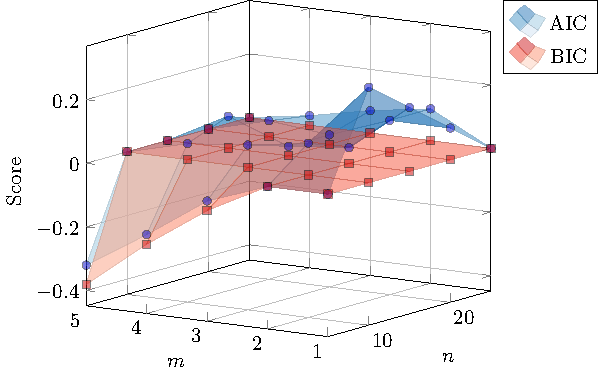
\includegraphics[width=\linewidth]{fig/nm.pdf}
            \caption{$n$--$m$ 平均得分统计图}\label{fig:nm}
        \end{minipage}
        \begin{minipage}[b]{.5\linewidth}
            \centering
            \captionof{table}{参数范围}
            \begin{tabular}{cl}
                \toprule
                类型 & 范围 \\
                \midrule
                $n$ & [5,10,15,20,25] \\
                $m$ & [1,2,3,4,5] \\
                随机种子个数 & 10 \\
                \midrule
                样本数量 $N$ & 200 \\
                噪声方差 $\sigma^2$ & 0.1 \\
                \bottomrule
            \end{tabular}
        \end{minipage}
    \end{figure}

    如图 \ref{fig:nm} 所示,对于不同的 $(n,m)$ 二元组,在 $m$ 比较大 $n$ 比较小时(左下角),AIC 和 BIC 预测表现都比较差,但是 AIC 略胜一筹;而 $m$比较小和 $n$ 比较大的时候(右上角),BIC 表现就比较好,AIC 往往会预测得略高一些。可见 AIC 更适合因素较多的时候,而 BIC 更适合因素单一的情况。

    \begin{figure}
        \begin{minipage}[c]{.5\linewidth}
            \centering
            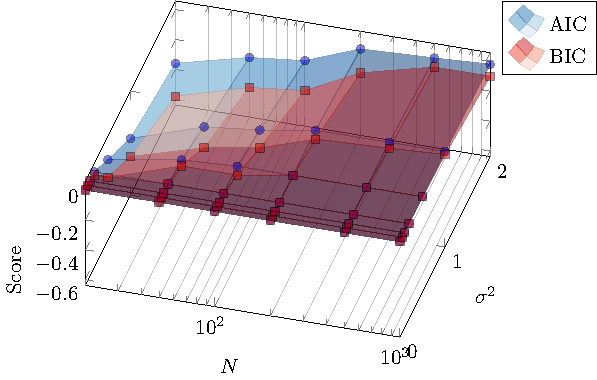
\includegraphics[width=\linewidth]{fig/Ns.pdf}
            \caption{$N$--$\sigma^2$ 平均得分统计图}\label{fig:Ns}
        \end{minipage}
        \begin{minipage}[b]{.5\linewidth}
            \centering
            \captionof{table}{参数范围}
            \begin{tabular}{cl}
                \toprule
                类型 & 范围 \\
                \midrule
                样本数量 $N$ & [20, 50, 100, 200, 500, 1000] \\
                噪声方差 $\sigma^2$ & [0, 0.05, 0.1, 0.2, 0.5, 1, 2] \\
                随机种子个数 & 10 \\
                \midrule
                $n$ & 10 \\
                $m$ & 5 \\
                \bottomrule
            \end{tabular}
        \end{minipage}
    \end{figure}

    如图 \ref{fig:Ns} 所示,对于不同的 $(N,\sigma^2)$ 二元组,在这个范围内,AIC 都要比 BIC 要好一些(主要是 $m$ 比较大,在上一点已论证),而样本数量越少,噪声越大(左上角),两者表现就会越差,会预测出较少的因素,BIC 的表现会下降得更快一些。

    \subsection{模型选择小结}

    单一元素情况,BIC 更好一些;多元情况,AIC 更好一些。样本数量越多,噪声越小,模型选择的表现就越好。

\end{document}